\documentclass[journal,12pt,twocolumn]{IEEEtran}

\usepackage{setspace}
\usepackage{gensymb}
\singlespacing


\usepackage[cmex10]{amsmath}
\newcommand{\norm}[1]{\left\lVert#1\right\rVert}
\usepackage{amsthm}

\usepackage{mathrsfs}
\usepackage{txfonts}
\usepackage{stfloats}
\usepackage{bm}
\usepackage{cite}
\usepackage{cases}
\usepackage{subfig}

\usepackage{longtable}
\usepackage{multirow}

\usepackage{enumitem}
\usepackage{mathtools}
\usepackage{steinmetz}
\usepackage{tikz}
\usepackage{circuitikz}
\usepackage{verbatim}
\usepackage{tfrupee}
\usepackage[breaklinks=true]{hyperref}
\usepackage{graphicx}
\usepackage{tkz-euclide}
\usepackage{float}

\usetikzlibrary{calc,math}
\usepackage{listings}
    \usepackage{color}                                            %%
    \usepackage{array}                                            %%
    \usepackage{longtable}                                        %%
    \usepackage{calc}                                             %%
    \usepackage{multirow}                                         %%
    \usepackage{hhline}                                           %%
    \usepackage{ifthen}                                           %%
    \usepackage{lscape}     
\usepackage{multicol}
\usepackage{chngcntr}

\DeclareMathOperator*{\Res}{Res}

\renewcommand\thesection{\arabic{section}}
\renewcommand\thesubsection{\thesection.\arabic{subsection}}
\renewcommand\thesubsubsection{\thesubsection.\arabic{subsubsection}}

\renewcommand\thesectiondis{\arabic{section}}
\renewcommand\thesubsectiondis{\thesectiondis.\arabic{subsection}}
\renewcommand\thesubsubsectiondis{\thesubsectiondis.\arabic{subsubsection}}


\hyphenation{op-tical net-works semi-conduc-tor}
\def\inputGnumericTable{}                                 %%

\lstset{
%language=C,
frame=single, 
breaklines=true,
columns=fullflexible
}
\begin{document}


\newtheorem{theorem}{Theorem}[section]
\newtheorem{problem}{Problem}
\newtheorem{proposition}{Proposition}[section]
\newtheorem{lemma}{Lemma}[section]
\newtheorem{corollary}[theorem]{Corollary}
\newtheorem{example}{Example}[section]
\newtheorem{definition}[problem]{Definition}

\newcommand{\BEQA}{\begin{eqnarray}}
\newcommand{\EEQA}{\end{eqnarray}}
\newcommand{\define}{\stackrel{\triangle}{=}}
\newcommand\hlight[1]{\tikz[overlay, remember picture,baseline=-\the\dimexpr\fontdimen22\textfont2\relax]\node[rectangle,fill=blue!50,rounded corners,fill opacity = 0.2,draw,thick,text opacity =1] {$#1$};}
\bibliographystyle{IEEEtran}
\providecommand{\mbf}{\mathbf}
\providecommand{\pr}[1]{\ensuremath{\Pr\left(#1\right)}}
\providecommand{\qfunc}[1]{\ensuremath{Q\left(#1\right)}}
\providecommand{\sbrak}[1]{\ensuremath{{}\left[#1\right]}}
\providecommand{\lsbrak}[1]{\ensuremath{{}\left[#1\right.}}
\providecommand{\rsbrak}[1]{\ensuremath{{}\left.#1\right]}}
\providecommand{\brak}[1]{\ensuremath{\left(#1\right)}}
\providecommand{\lbrak}[1]{\ensuremath{\left(#1\right.}}
\providecommand{\rbrak}[1]{\ensuremath{\left.#1\right)}}
\providecommand{\cbrak}[1]{\ensuremath{\left\{#1\right\}}}
\providecommand{\lcbrak}[1]{\ensuremath{\left\{#1\right.}}
\providecommand{\rcbrak}[1]{\ensuremath{\left.#1\right\}}}
\theoremstyle{remark}
\newtheorem{rem}{Remark}
\newcommand{\sgn}{\mathop{\mathrm{sgn}}}
\providecommand{\abs}[1]{\left\vert#1\right\vert}
\providecommand{\res}[1]{\Res\displaylimits_{#1}} 
\providecommand{\norm}[1]{$\left\lVert#1\right\rVert$}
%\providecommand{\norm}[1]{\lVert#1\rVert}
\providecommand{\mtx}[1]{\mathbf{#1}}
\providecommand{\mean}[1]{E\left[ #1 \right]}
\providecommand{\fourier}{\overset{\mathcal{F}}{ \rightleftharpoons}}
%\providecommand{\hilbert}{\overset{\mathcal{H}}{ \rightleftharpoons}}
\providecommand{\system}{\overset{\mathcal{H}}{ \longleftrightarrow}}
	%\newcommand{\solution}[2]{\textbf{Solution:}{#1}}
\newcommand{\solution}{\noindent \textbf{Solution: }}
\newcommand{\cosec}{\,\text{cosec}\,}
\providecommand{\dec}[2]{\ensuremath{\overset{#1}{\underset{#2}{\gtrless}}}}
\newcommand{\myvec}[1]{\ensuremath{\begin{pmatrix}#1\end{pmatrix}}}
\newcommand{\mydet}[1]{\ensuremath{\begin{vmatrix}#1\end{vmatrix}}}
\numberwithin{equation}{subsection}
\makeatletter
\@addtoreset{figure}{problem}
\makeatother
\let\StandardTheFigure\thefigure
\let\vec\mathbf
\renewcommand{\thefigure}{\theproblem}
\def\putbox#1#2#3{\makebox[0in][l]{\makebox[#1][l]{}\raisebox{\baselineskip}[0in][0in]{\raisebox{#2}[0in][0in]{#3}}}}
     \def\rightbox#1{\makebox[0in][r]{#1}}
     \def\centbox#1{\makebox[0in]{#1}}
     \def\topbox#1{\raisebox{-\baselineskip}[0in][0in]{#1}}
     \def\midbox#1{\raisebox{-0.5\baselineskip}[0in][0in]{#1}}
\vspace{3cm}
\title{Assignment No.3}
\author{RajaSekhar Jala}
\maketitle
\newpage
\bigskip
\renewcommand{\thefigure}{\theenumi}
\renewcommand{\thetable}{\theenumi}
Download all python codes from 
\begin{lstlisting}
https://github.com/Sekharjala/Assignment_3/codes
\end{lstlisting}
%
and pdf from 
%
\begin{lstlisting}
https://github.com/Sekharjala/Assignment_3/Assignment3.pdf
\end{lstlisting}
%
\section{Quadratic Forms Q:2.5}
Question :
Find the area of the region in the first quadrant enclosed by x-axis, line $\myvec{1 & -\sqrt{3}}\vec{x} =0$ and the circle \vec{x}^T\vec{x}=4

\section{Solution}
Given equation of a circle is 
    \begin{align}
        \vec{x}^{T} \vec{x} =4 \label{eq:A}
    \end{align}
can be expressed as,
\begin{align}
    \vec{x}^{T}\vec{x} - 2\vec{u}^{T}\vec{x} +f=0 \label{eq:eq1}
\end{align}
where $\vec{c}$ is the center.\\
Comparing equation \eqref{eq:eq1} with the circle equation given,
\begin{align}
    \vec{x}^{T}\vec{x} =4 \label{eq:eq2}\\
    \quad f = \vec{u}^T \vec{u}-r^2 \\
    \implies \vec{c} = \myvec{0\\0} \quad f=-4\\
    r=\sqrt{\vec{u}^{T}\vec{u}-f} = \sqrt{4}\\
    r=2 \label{eq:eq3}
\end{align}
From equation \eqref{eq:eq3}, circle is having center at \vec{0 \\ 0} with radius of 2 units.The equation of the diagnal is  $x$-axis is and the directional vector is 
\begin{align}
    \myvec{2 \\ 0} - \myvec{0 \\ 0} = \myvec{2 \\ 0}    
\end{align}
The direction vector of line formed with \vec{O} and \vec{A} is  $\myvec{2\\0}$.\\
The direction vector of the given line 
\begin{align}
    \myvec{1&-\sqrt{3}}\vec{x}=0 is \myvec{\sqrt{3}\\1} \label{eq:eqA}
\end{align}
The angle between line \eqref{eq:eqA} with \vec{OA} ,
\begin{align}
    \cos\theta = \frac{\myvec{\sqrt{3}&1}\myvec{2\\0}}{\norm{\myvec{\sqrt{3}&1}}\norm{\myvec{2&0}}}=\frac{\sqrt{3}}{2} \label{eq:solutions/7/eq:eq4}\\
    \theta = 30^{\degree}\label{eq:eq5}
\end{align}
Using equation \eqref{eq:eq3} and \eqref{eq:eq5},the area of the sector is obtained as,
\begin{align}
    \frac{\theta}{360^{\circ}}\pi r^2 = \frac{30^{\circ}}{360^{\circ}}\pi (2)^2=\frac{\pi}{3} \label{eq:eq6}
\end{align}

\begin{figure}[H]
\centering
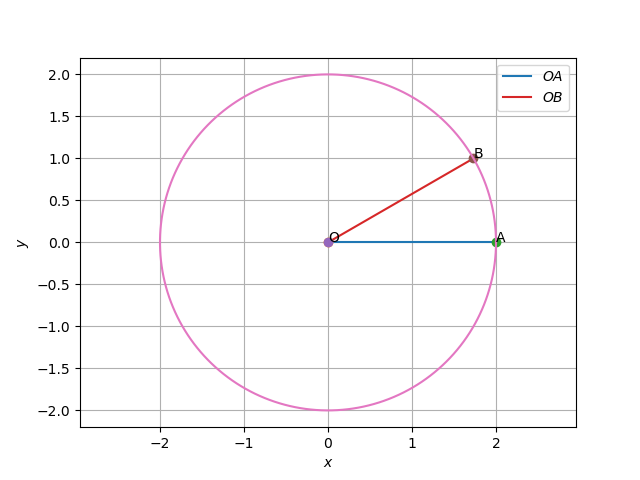
\includegraphics[width=\columnwidth]{circle.png}
\caption{Area Under the Curve & circle  }
\label{fig:1}
\end{figure}
Ref:Tangents & Normals \\
If a line 
\begin{align}
    L:  \vec{x} = \vec{a} + \lambda \vec{m} 
\end{align}
touches a conic section at one point $\vec{q}$ then
\begin{align}
\vec{m}^T(\vec{V} \vec{q}+\vec{u}) = 0  \label{eq:EqP}
\end{align}
From equation \eqref{eq:A} $\Vec{V}$ is \myvec{1&0 \\ 0&1}  and $\vec{u}$=\myvec{0 \\ 0}\\
from eq \eqref{eq:A} and \eqref{eq:EqP} point of intersection is $\Vec{A}$ is given by
\begin{align}
    \myvec{0 & 2} (\myvec{1&0\\0&1}\vec{A}+\vec{u})&=0 \\
    \myvec{0&2}\vec{A}&=0 \\
    \implies \vec{A}&=\myvec{2\\ 0} 
\end{align}
similarly \\
from eq \eqref{eq:eqA} and \eqref{eq:EqP} point of intersection is \Vec{B} is given by
\begin{align}
    \myvec{1 & -\sqrt{3}} (\myvec{1&0\\0&1}\vec{B}+\vec{u})&=0 \\
    \myvec{1 & -\sqrt{3}}\vec{B}&=0 \\
    \implies \vec{B}&=\myvec{\sqrt{3} \\ 1 } 
\end{align}
% Point $\vec{A}$ = \myvec{2 \\ 0} \\
% Point $\vec{B}$ is on the line \myvec{1&-\sqrt{3}}\vec{x}=0 can be expressed as
% \begin{align}
%   \vec{x}=\vec{p}+\lambda \vec{m} 
% \end{align}
%  Where \vec{p} is a vector and \vec{m} is Directional vector of the line
% \begin{align}
%     \vec{x}=\myvec{0 \\ 0}+ \lambda \myvec{\sqrt{3} \\ 1} \label{eq:eq7}
% \end{align}
% from \eqref{eq:A} substituting value of \vec{x} we get
% \begin{align}
% {\myvec{{\myvec{0 \\ 0}+ \lambda \myvec{\sqrt{3} \\ 1}}} ^T \myvec{ \myvec{0 \\ 0}+ \lambda \myvec{\sqrt{3} \\ 1}}} =4 \\
% \lambda \myvec{\sqrt{3} & 1} \times \lambda \myvec{\sqrt{3} \\ 1}=4 \\
% \lambda ^2  \myvec{4} =4 \\    
% \lambda =1 \label{eq:eq8}
% \end{align}
% substitute \eqref{eq:eq8} in \eqref{eq:eq7} point on circle
% \begin{align}
%     \vec{x}=\myvec{0 \\ 0}+ \lambda \myvec{\sqrt{3} \\ 1} \\
%     \vec{x}=\myvec{0 \\ 0}+ 1 \myvec{\sqrt{3} \\ 1} \\
%     \vec{x}= \myvec{\sqrt{3} \\ 1}
% \end{align}

\end{document}
